\subsection{Peak Ratio}
\label{subsec:peakratio}

To further examine difference
%We suggest that the FCC adopt multiple benchmarks to better characterize broadband availability, deployment, and adoption in the US, based on our analysis of varying usage patterns within the same ISP tier.
%We explore a taxonomy of different users based on varying traffic patterns of users within the same capacity tier, and 


\hypoth{4}. How much does the traffic vary in a single day?

\begin{itemize}
\itemsep0em 
\item Figure ~\ref{fig:CDF-peak-ratio-median}
\item test-set sees higher variance in usage per device
\item implies that ISPs should condition their networks to 50 times median usage per user
\end{itemize}


%%%%%%%%%%%%%%%%%%%%%%%%%%%%%%%%%%%%%%%%%%%%%%%%%%%%%%%%%%%%%%%%%%%%%

\begin{figure}[ht!]
\begin{minipage}{0.90\linewidth}
\centering
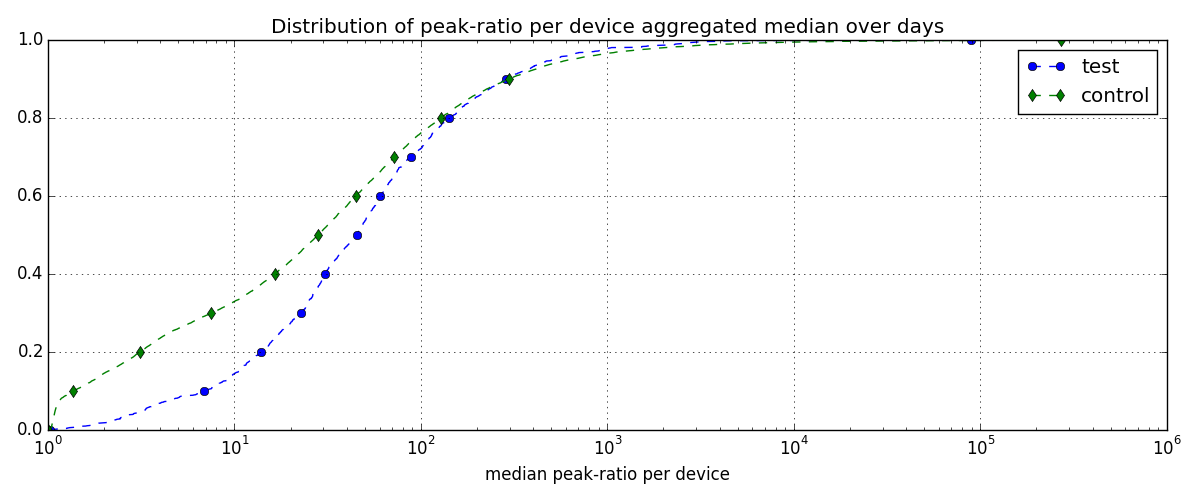
\includegraphics[width=1\linewidth]{figures/peakratio-CDF-devices-MEDIAN.png}
\caption{Median peak ratio per device showing that test set has higher daily variance, which goes upto 50 times)}
%http://sites.noise.gatech.edu/~sarthak/files/comcast/plots/full_dw/peakratio-CDF-devices-MEDIAN.png
\label{fig:CDF-peak-ratio-median}
\end{minipage}
\end{figure}



%%%%%%%%%%%%%%%%%%%%%%%%%%%%%%%%%%%%%%%%%%%%%%%%%%%%%%%%%%%%%%%%%%%%%





%
%big difference (2 x median ratio) in per device per day ratios of 90%ile:median.
%weird shape again for values < ratio 100
%big difference in this ratio per day, and it is consistent across all individual sets + months.
%very large for Dec, slightly smaller for Nov
%interestingly, at higher ratios control is slightly > test. This means that certain devices in control set have a huge std (ratio) in a day as compared to test set which has a lower “max” ratio.
%

